\chapter{Results II --- Co-design and the Capacity Envelope}\label{ch:codesign}

\needswork{STATUS: DRAFTED. The ablation section deliberately narrows the thesis's own claim.}

\section{E5 --- the end-to-end configuration}

Exhaustive search over the full grid returns delta-CBOR, Ed25519, placement B, $b = 4$: $72.0$\,B
per record against $174.3$\,B for the compression-only baseline and $299.1$\,B for the naive one ---
a \textbf{$58.7\%$ total-byte reduction}.

\begin{remark}[Report the decomposition, never the bare authentication ratio]
The authentication-byte cut is $75.0\%$, and it is tempting to lead with it. It must not be led with,
because it reduces algebraically to $1 - 1/b$: invariant to the header, the signature size, the
encoding and the scheme. It is the definition of batching, not a result. The honest headline is the
\emph{total} byte reduction reported as a decomposition --- placement$\times$batching $79.2\%$,
encoding $20.8\%$, scheme byte-neutral.
\end{remark}

\begin{figure}[h]
\centering

\includegraphics[width=0.7\textwidth]{fig_e5_codesign.png}
\caption{End-to-end per-record cost against the two baselines.}
\label{fig:e5}
\end{figure}

\section{The factorial ablation, which narrows the claim}

A full factorial ablation over the four axes asks whether ``co-design'' is doing work that
single-axis optimisation would not.

\begin{itemize}
\item \textbf{Placement and batching couple exactly}, by $\ga(1 - 1/b)$ --- hence \emph{exactly
      zero} at $b = 1$, where placements A and B are byte-identical on a single-record frame.
\item \textbf{Encoding is perfectly separable.} Every interaction term is exactly zero, because $s$
      enters additively and therefore \emph{cannot} interact.
\item \textbf{The scheme axis is byte-degenerate} in this regime: the two $64$\,B schemes differ
      only in CPU cost.
\end{itemize}

An earlier claim that a smaller payload increases the value of batching was a \textbf{ratio-scale
artifact}: the absolute saving is $81.0$\,B for every encoding. The four-axis co-design claim was
overstated and is now precise. \textbf{No number moved --- only its interpretation.}

\begin{remark}
Note that $1 - 1/b$ is the same term as the warning above. The genuine coupling and the flattering
headline are the same algebra, seen from two directions.
\end{remark}

\section{E4 --- scheme selection on real hardware}

On ARM --- the deployment platform --- Ed25519 verification is $33.2\times$ cheaper than a BLS
pairing, which keeps Ed25519 optimal for self-batching at any plausible radio/CPU power ratio. The
ordering between Ed25519 and ECDSA-P256 \emph{flips} between x86 and ARM, so the choice is
platform-specific; the authentication-byte result is identical either way, since both are $64$\,B.

\begin{figure}[h]
\centering
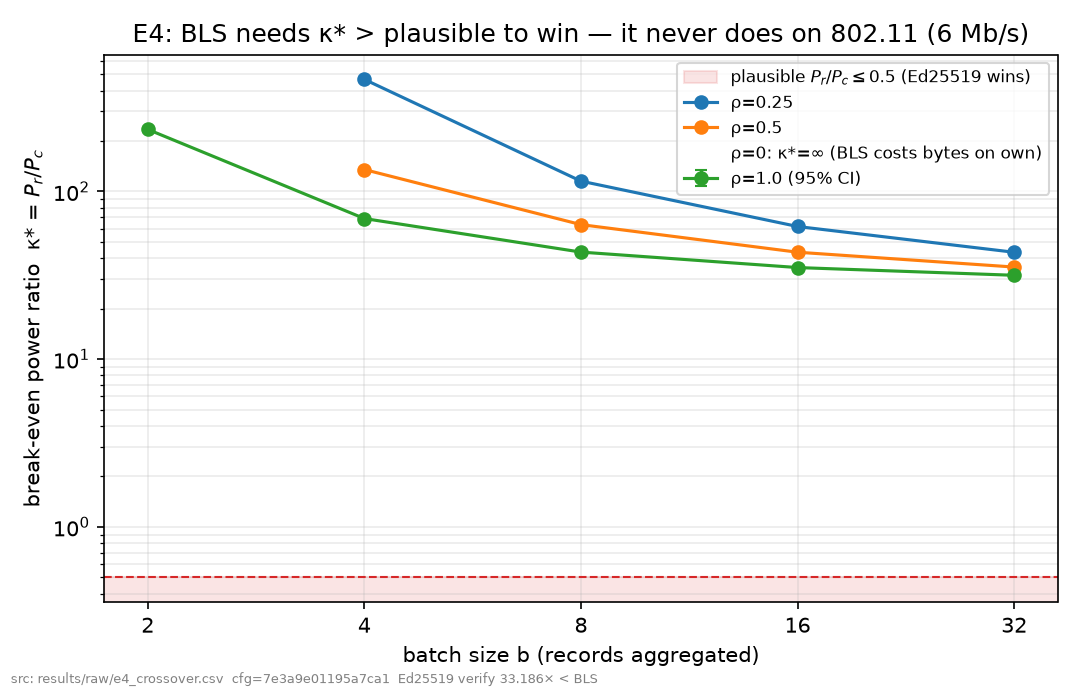
\includegraphics[width=0.7\textwidth]{e4_crossover.png}
\caption{The scheme crossover. BLS becomes worthwhile only in the cross-signer regime.}
\label{fig:e4}
\end{figure}

\section{E8 --- the capacity envelope}

Joining the byte model to the validated broadcast channel model turns ``how many bytes?'' into the
question an operator actually asks: \emph{how many UAVs, at what telemetry rate?}

\begin{table}[h]
\centering
\caption{Largest sustainable neighbourhood, reported at two thresholds because they answer
different questions. The per-run column is the reliability reading of the same criterion.}
\label{tab:envelope}
\begin{tabular}{lrrrrrr}
\toprule
configuration & $\Lambda_i$ & $\Dmax$ & $b$ & $\Nmax$ ($U{<}1$) & $\Nmax$ ($V$ mean) & ($V$ per run) \\
\midrule
\multicolumn{7}{l}{\emph{Primary: compliant with 3GPP TS 22.125}}\\
\textbf{optimized} delta/B & 50 & 100\,ms & 4 & \textbf{35} & \textbf{100} & 64--91 \\
A+CBOR (compression-only)  & 50 & 100\,ms & 1 & 18 & 31 & 24--29 \\
\midrule
\multicolumn{7}{l}{\emph{Relaxed freshness: same bytes, larger swarm, exceeds the standard}}\\
optimized delta/B & 20 & 250\,ms & 4 & 103 & 213 & 163--201 \\
A+CBOR            & 20 & 250\,ms & 1 & 32  & 88  & 54--80 \\
\bottomrule
\end{tabular}
\end{table}

The four ratios are $1.94\times$, $3.23\times$, $3.22\times$ and $2.42\times$.

\begin{remark}[Do not round this to ``about three times'']
The spread is $1.9$--$3.2\times$ and must be quoted as a range. An earlier draft of this work said
``$\approx 3\times$ holds across readings'', which is both false and precisely the kind of claim the
rest of this thesis exists to avoid. The co-design advantage is \emph{insensitive to the choice of
threshold} --- that is the defensible statement --- but it is not a single number.
\end{remark}

\begin{figure}[h]
\centering

\includegraphics[width=0.75\textwidth]{fig_envelope.png}
\caption{The feasibility envelope. The compression-only baseline runs out of channel where the
co-designed configuration does not.}
\label{fig:envelope}
\end{figure}

\section{What the envelope rests on}

The absolute capacities depend on a utilisation ceiling measured at one operating point and applied
across the envelope. \Cref{ch:validation} reports the experiment that tested that assumption, and
what it still leaves untested. The \emph{ratios} are protected by construction, because numerator
and denominator use the same ceiling; the absolute figures are not, which is why both are given.
